\section{Bioetica 2: Il Rischio Clinico}

Il rischio clinico è un tema molto importante in qualsiasi ambito della
medicina, perché solo ponendoci il problema del perché qualcosa sia
andato storto riusciamo a sbagliare meno.

Questa cultura serve ad attenuare l'arroganza culturale della nostra
categoria, ad imparare a lavorare insieme e a sbagliare di meno. È bene
considerare come il nostro mestiere anni fa fosse ``solitario'', mentre
oggi si è obbligati a lavorare con altre figure professionali, anche
facendo il medico di famiglia si entra a contatto con segretarie,
infermiere domiciliari, infermiere nello studio\ldots{} Nonostante non
sia come per l'anestesista che lavora in equipe, in ogni caso con ognuno
di queste figure va trovata una modalità di lavoro.

Il rischio clinico è inserito nell'ambito della deontologia medica
perché l'atteggiamento finalizzato al bene del paziente e della comunità
dev'essere il fine supremo del nostro mestiere. Tutto quello che
facciamo, compresi i tentativi di ridurre i possibili errori, è in
funzione di ottenere il massimo della qualità professionale che possiamo
esprimere.

Il SSN è un sistema complesso, integrato, e deve avere delle procedure
di sicurezza, che vanno dalle vie di fuga sul posto di lavoro, ai
sistemi antincendio, fino alla necessità di valutare preliminarmente il
rischio a cui andiamo incontro. La necessità di avere l'alleanza
diagnostica e terapeutica col paziente passa attraverso una valutazione
preliminare di quelli che sono i rischi e benefici dell'attività che
andiamo a proporre, confrontandoci con quella che è la pseudo-conoscenza
che il paziente può avere. L'atto della firma del consenso informato
sembra spesso una pratica assicurativa, facendo firmare ai pazienti cose
che non sempre capiscono.

Sappiamo che un paziente porta a casa il 10\% di quello che si dice a
colloquio, quindi è solo spendendo del tempo a spiegare i motivi per i
quali è utile fare una certa attività che avremo il consenso e una
valutazione congiunta del rischio-beneficio. Nella misura in cui
riusciamo a condividere col paziente i problemi, questo capirà e non
creerà dei retropensieri, scongiurando il contenzioso medico.

In un sistema complesso perciò è fondamentale slatentizzare le
situazioni critiche per ottenere maggiore sicurezza possibile.

Bisogna ricordare che la \emph{percentuale di danni iatrogeni causati} è
diventato un indicatore della qualità delle cure. Nel momento in cui
qualcosa non funziona andiamo sempre a chiederci il perché, dove abbiamo
sbagliato, che cosa si poteva fare e che cosa potremmo fare per evitare
che succeda di nuovo. In sintesi significa attuare una \emph{revisione
critica sistematica} dei propri comportamenti allo scopo di ``sbagliare
un po' meno''.

La maggior parte degli errori che si fanno è spesso imputabile alla
velocità e la ripetitività dei gesti, i ritmi di lavoro (fare più cose
contemporaneamente). Andare a cercare il meccanismo con cui si sono
prodotti degli errori ci serve per sbagliare di meno la volta
successiva.

\subsection{Definizione}

\textbf{Rischio clinico}\emph{: possibilità per un paziente di subire un
danno o un disagio grave, che per definizione si presume involontario,
legato ed imputabile alle cure sanitarie e che determina un
prolungamento delle stesse cure, cui consegue un aumento dei tempi di
degenza ospedaliera, un peggioramento del suo stato di salute, che
arriva a tale compromissione da portare fino alla morte.}

Qualsiasi tipo di danno prodotto in modo involontario è il motivo della
valutazione che deve stare alla base del rischio clinico. Il rischio
clinico rappresenta il pericolo che il gesto professionale che noi
facciamo possa provocare un danno al paziente. Sempre ricordando che
anche lo stesso ricovero in ospedale è di per sé un motivo di rischio,
ad esempio di infezione (uso di cateteri vescicali, piaghe da
decubito...).

Un problema frequente in ambiente medico è l'autoreferenzialità. Bisogna
cercare di evitare di essere supponenti e autoreferenziali. Solo
l'ascolto e la risposta ai problemi dei pazienti porta a una
\emph{alleanza terapeutica}. Il prof riporta a proposito di come lui
stesso utilizzi molto dei disegni per aiutarsi nella spiegazione ai
pazienti.

\begin{figure}[!ht]
\centering
	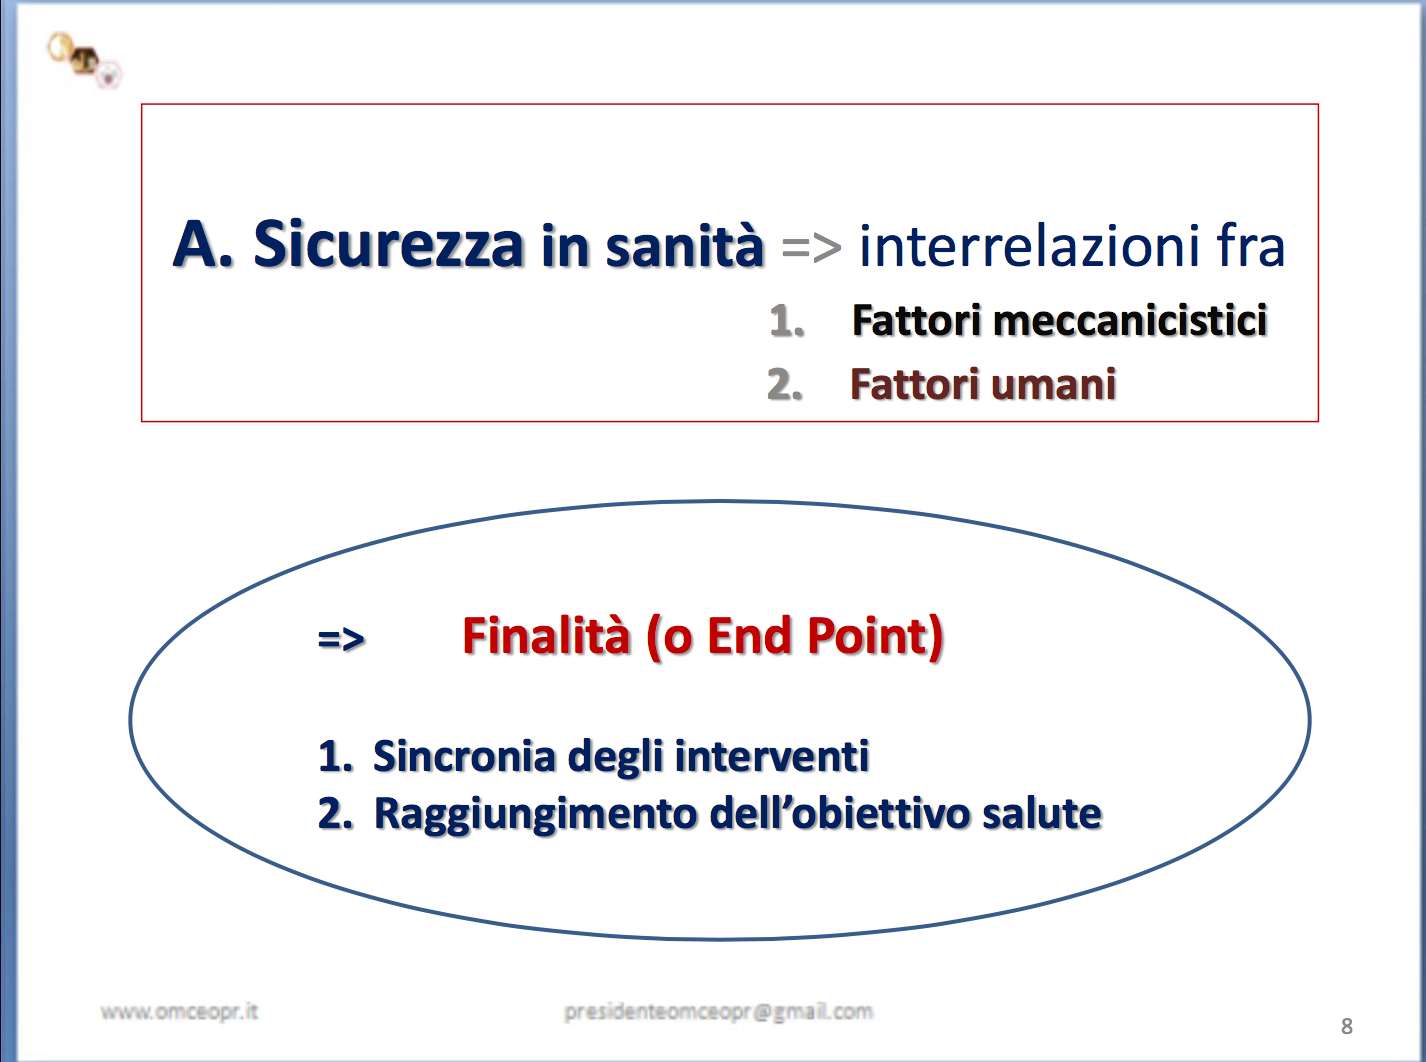
\includegraphics[width=0.8\textwidth]{30/image1.png}
	\end{figure}

\subsection{La sicurezza}

La sicurezza dipende da fattori meccanicistici e fattori umani. Quindi
non dipende solo dalla competenza del medico, dalla sua predisposizione,
ma anche da fattori organizzativi e gestionali che spesso non dipendono
soltanto da esso.

La cultura della sicurezza va perseguita attraverso:

\begin{itemize}
\item[1.]
  \textbf{Competenza:} conoscenza dei fattori tecnici, organizzativi,
  ambientali e umani, ma anche dei possibili errori. Importante
  conoscere non solo ciò che c'è da sapere, ma anche dove è possibile
  sbagliare.
\item[2.]
  \textbf{Equità:} consapevolezza e fiducia nella corretta segnalazione
  delle variabilità che portano all'errore. È giusto ed equo essere
  sempre nell'atteggiamento mentale di segnalare ciò che non va, questo
  da parte di tutti i membri di un'equipe. Es infermiera che segnala un
  callo possibilmente soggetto a infezione in un piede diabetico.
\item[3.]
  \textbf{Chiarezza nella segnalazione} degli errori e delle situazioni
  potenzialmente nocive che possano determinarli.
\item[4.]
  \textbf{Flessibilità}: capacità e responsabilità nell'adottare le
  soluzioni. Capacità di adattarsi.
\end{itemize}

Avendo capito che l'errore in sanità esiste, e che è sia possibile che
probabile, quando accade occorre valutare:

\begin{itemize}
\item[1.]
  Causa diretta o indiretta
\item[2.]
  Insufficienza organizzativa (es la fretta, fare più cose
  contemporaneamente)
\item[3.]
  Errore umano
\item[4.]
  Non rispetto della prassi e/o dei protocolli
\item[5.]
  Distrazione
\item[6.]
  Incidente di percorso
\item[7.]
  Grado di imponderabilità.
\end{itemize}

Fare una \emph{\textbf{check-list}} può aiutare a ripercorrere quello
che si dovrebbe fare e ridurre il rischio d'errore da ripetitività, che
è uno dei più frequenti.

\subsection{Glossario utile}

\begin{itemize}
\item[1.]
  \textbf{Danno}: alterazione temporanea o permanente di una parte del
  corpo o di una funzione psico-fisica.\\
  È quello che ci infelicità molto spesso l'esistenza, perché quando
  qualcuno ritiene di aver subito un danno, fa denuncia.
\item[2.]
  \textbf{Errore}: alterato compimento di azione o procedura nel
  raggiungimento dell'obiettivo prefissato.
\item[3.]
  \textbf{Evento sfavorevole}: evento che che produce un incidente
  legato al danno. Voluto o non voluto / preventivabile o non
  preventivabile, comunque non intenzionale.
\item[4.]
  \textbf{Evento:} meglio definito come normale esito di procedura
  (\textbf{E. favorevole)} ma anche incidente legato a danno voluto/non
  voluto, preventivabile o non preventivabile (\textbf{E. sfavorevole).}
\item[5.]
  \textbf{Evento avverso:} evento inatteso, indesiderato ed
  indesiderabile, prevedibile solo in caso di errore.
\item[6.]
  \textbf{Evento avverso evitato} (o near miss): evento non comparso per
  causa fortuita o per accuratezza del controllo, con intercetto della
  procedura eventualmente errata.\\
  È quello che dovremmo cercare di ottenere.
\item[7.]
  \textbf{Evento sentinella}: evento sfavorevole indice di
  malfunzionamento della struttura o della nostra preparazione. Deve
  essere corretto in quanto è fonte di ripetizione dell'errore.
\item[8.]
  Il \textbf{governo clinico} è quella braca della medicina che si
  occupa della gestione delle forze sanitarie per la limitazione degli
  eventi sfavorevoli e per il miglioramento del sistema sanitario.
\item[9.]
  \textbf{Rischio}: situazione potenziale di evento avverso.
\end{itemize}

\subsection{Errore}

\begin{itemize}
\item
  \textbf{Errore attivo}: prodotto direttamente da una pratica errata,
  ad esempio una toracentesi che produce uno pneumotorace;
\item
  \textbf{Errore latente}: situazione che prelude e che può portare
  all'errore. Sono insufficienze di sistema di tipo
  organizzativo-gestionale che determinano un errore attivo.
\end{itemize}

L'errore comporta una serie di ``deficit protettivi nel sistema
organizzativo. Le \textbf{falle di sistema} sono situazioni che se non
colte preliminarmente possono portare a una successione di errori fino
ad ottenere l'evento più disastroso.

Per \emph{pignoleria dell'analisi} si intende una mentalità incentrata
sul guardare sistematicamente, fare la check-list ad esempio.
Dall'analisi dell'errore si può ottenere una valutazione dei componenti
della struttura del sistema e della componente umana fonte dell'errore.
Dall'analisi dell'evento avverso, risalire al perché abbiamo sbagliato e
come possiamo evitare di sbagliare la volta successiva.

L'errore attivo è facilmente rilevabile, l'errore latente è molto più
subdolo, ed è conseguenza di una catena di eventi facilitanti, come
scelte sbagliate che facilitano il danno.

Ci sono diversi \emph{atteggiamenti} nei confronti dell'errore che noi
commettiamo. Fa parte dell'animo umano l'idea che nessuno ami ammettere
di aver sbagliato, nessuno lo fa con facilità e molto spesso l'errore ci
porta:

\begin{itemize}
\item[1.]
  A una fuga dalle responsabilità o all'attribuzione ad altri,
\item[2.]
  All'isolamento e angoscia per l'accaduto.
\end{itemize}

Solo costruendo una cultura diversa, basata sulla condivisione della
responsabilità e della valutazione dell'errore, in funzione della non
ripetizione, potremmo attenuare questi fenomeni.

Gestire il rischio clinico significa esorcizzare la paura di lavorare e
di commettere errori, agire per prevenire e per migliorare in sanità.

Quando andiamo a rilevare una criticità in una pratica che fa un
collega, andrebbe vissuto non come delazione, ma come strumento di
miglioramento. Pensare che la gestione del rischio sia finalizzata al
miglioramento e non alla colpevolizzazione aiuta ad avere un approccio
diverso nei confronti sia dei colleghi, che del problema che si è
creato.

\begin{figure}[!ht]
\centering
	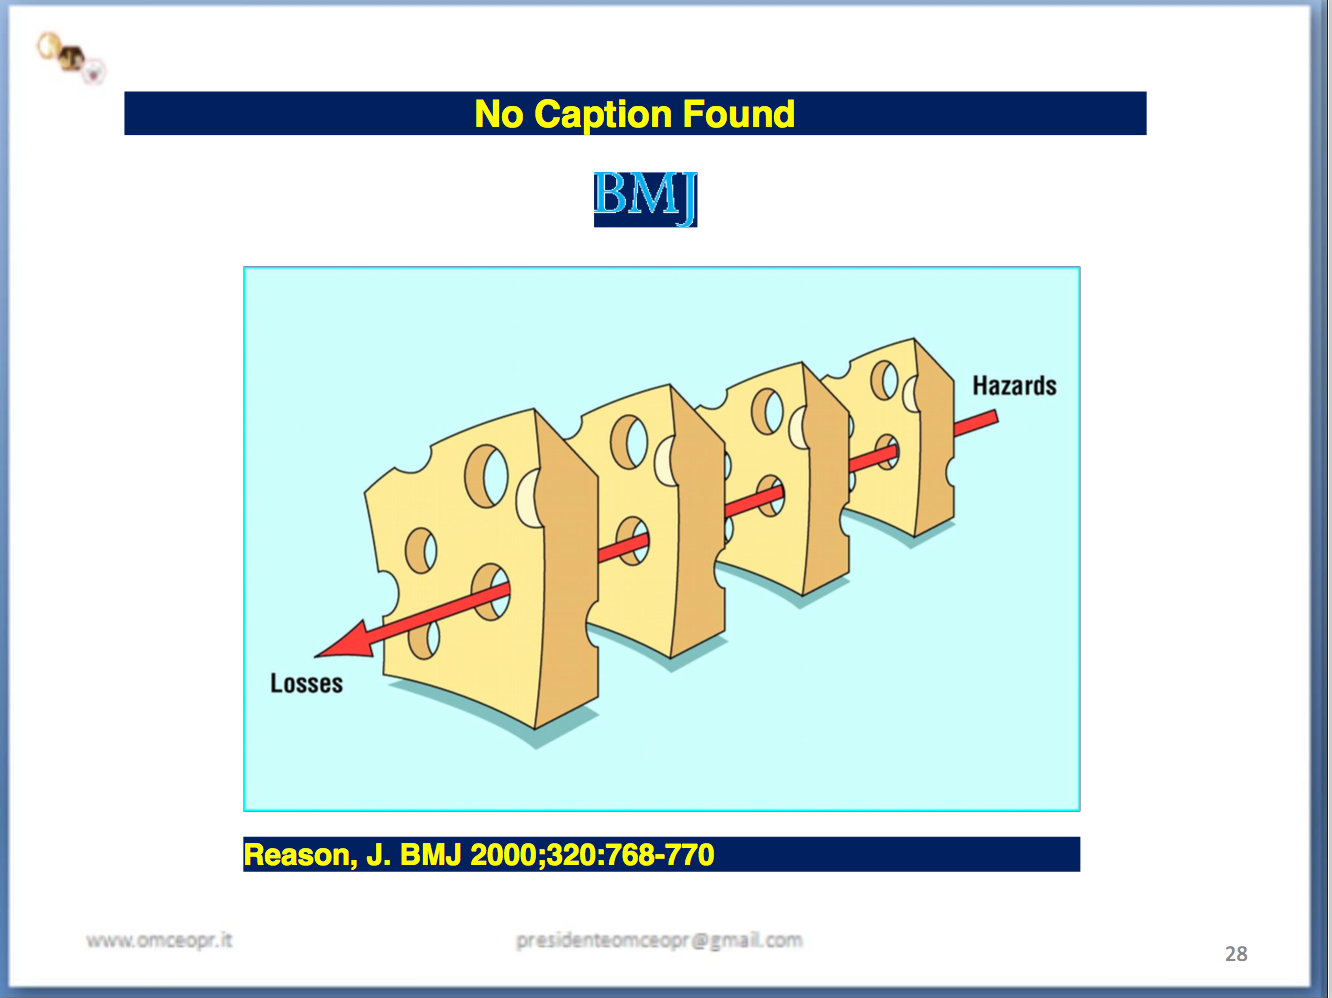
\includegraphics[width=0.8\textwidth]{30/image2.png}
	\end{figure}

La
connessione tra etica medica e gestione del rischio sta nell'avere un
approccio finalizzato a ottenere il meglio (sbagliare un po' meno),
perché l'etica è l'insieme delle azioni che devono guidare il medico a
ottenere il meglio per il paziente e per la comunità dove opera.

``Gli incidenti avvengono per interazione delle diverse componenti di un
sistema complesso''

Il prof sfrutta l'analogia della serie di errori e della responsabilità
individuale con i buchi del formaggio gruviera. Una serie di buchi in
sequenza rappresentano errori commessi in sequenza e mancanza di
segnalazione efficace da parte delle varie figure professionali che si
susseguono in un percorso medico. (Tesi del gruviera, J.Reason)
\\\\
Il \textbf{grado di rischiosità} si misura con:

\begin{itemize}
\item[1.]
  Fattori strutturali e tecnologici: es la non sterilità di una sala
  operatoria
\item[2.]
  Fattori organizzativo-gestionali e condizione di lavoro: es la fretta
\item[3.]
  Fattori umani (esecutori di prestazione): stanchezza, situazioni
  personali\ldots{}
\item[4.]
  Fattori umani (destinatari di prestazione=paziente)
\item[5.]
  Fattori esterni
\end{itemize}

\begin{figure}[!ht]
\centering
	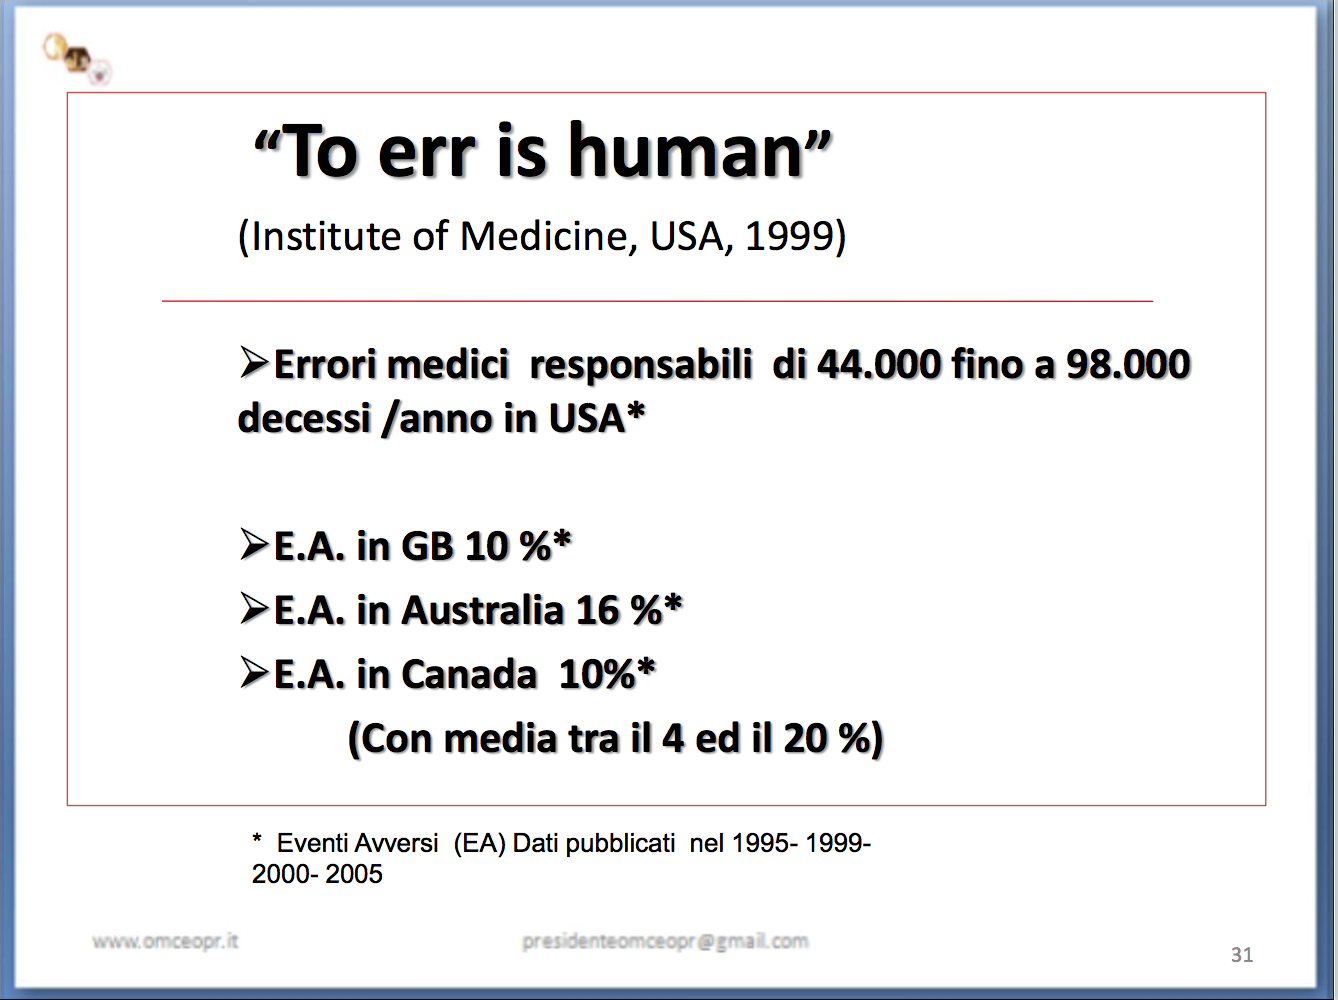
\includegraphics[width=0.8\textwidth]{30/image3.png}
	\end{figure}

La
\emph{cultura del rischio}: l'errore è sempre possibile per cui si deve
preventivamente analizzare il meccanismo o i meccanismi che lo possano
determinare attuando un'efficace prevenzione. \emph{``se lo conosci lo
eviti''}

Conosciuto l'errore cosa fare?

\begin{itemize}
\item
  Conoscere ciò che si fa a livello internazionale nelle varie comunità
  sanitarie (USA, mondo anglosassone, Europa), ciò che la comunità
  scientifica condivide come cosa migliore, le linee guida.
\item
  Attivare le procedure di analisi e di intervento previste per la
  prevenzione e la gestione del rischio clinico (programmazione e
  controllo sanitario).
\end{itemize}

\subsection{Procedure consigliate (management)}

\begin{itemize}
\item[1.]
  \emph{Sperimentazione} di modelli organizzativi e tecnologie avanzate,
  ottimizzanti la gestione e la comunicazione (semplificazione).
\item[2.]
  \emph{Determinazione} di procedure: per la riduzione dell'errore.
\item[3.]
  \emph{Diffusione} della cultura della prevenzione dell'errore
  attraverso eventi formativi ad hoc.
\item[4.]
  \emph{Elaborazione} delle raccomandazioni per la prevenzione degli
  ``eventi sentinella''.
\item[5.]
  \emph{Elaborazione} dei percorsi e linee guida per l'evidenza omogenea
  degli errori e dei rischi.
\item[6.]
  \emph{Promozione} della segnalazione dei ``quasi errori'' o near miss
  e degli ``eventi sentinella''.\\
  Il prof tiene particolarmente a questo punto. Racconta pertanto un
  episodio accadutogli in merito a un paziente, che senza appuntamento
  si era presentato in ambulatorio per un dolore alla spalla, a seguito
  di una caduta durante una partita di calcetto. A causa di una serie di
  fattori personali (preconcetti, stress, situazione frenetica) il prof
  dice di aver eseguito un'eco al pz e di aver rilevato un ematoma
  nell'inserzione distale del bicipite brachiale, ma nessuno strappo
  tendineo. Segue invio del pz al fisioterapista per la terapia fisica.
  Il fisioterapista avrebbe poi rimandato al prof il pz perché in
  disaccordo con la diagnosi. Alla seconda osservazione, in effetti era
  evidente che ci fosse una lesione estesa del tendine. L'episodio è
  stato fonte di riflessione per capire quali fossero stati i fattori
  implicati nella genesi dell'errore, e come agire al fine di evitarli
  in futuro.
\item[7.]  \emph{Monitoraggio} periodico degli eventi e incentivazione della
  procedura di informazione puntuale e corretta.
\item[8.]
  \emph{Coordinamento} del sistema allargato di gestione del rischio
  clinico.\\
  Instillare la cultura del rischio clinico nelle persone che ci
  lavorano a fianco.
\item[9.]
  \emph{Sperimentazione} delle procedure di segnalazione, raccolta ed
  elaborazione dei dati relativi all'errore in caso di procedure ad alto
  rischio.
\item[10.]
  \emph{Coinvolgimento} nel processo dei parenti dei pazienti, dei
  cittadini e dei lavoratori impegnati a vario livello nella gestione
  del rischio. La firma del consenso informato dev'essere solo l'ultima
  parte di un contratto che prevede che il paziente abbia sviluppato
  consapevolezza e informazione su quello che è destinato a fare.
\end{itemize}

Riassumendo per punti principali l'analisi del controllo del rischio:

\begin{itemize}
\item[1.]
  Attivarsi per slatentizzare le situazioni che possono portare a un
  evento avverso.
\item[2.]
  Avere un \emph{approccio proattivo} (analisi dei percorsi e procedure
  con rilievo delle criticità) finalizzato alla prevenzione dell'evento
  sfavorevole.
\item[3.]
  \emph{Approccio reattivo} all'analisi dell'evento sfavorevole con
  identificazione dei fattori che lo hanno determinato.
\end{itemize}
Strumenti di identificazione del rischio:

\begin{itemize}
\item
  I \emph{sistemi di segnalazione} sono sezioni del governo clinico che
  fanno un reporting degli errori che possono essere stati fatti in un
  determinato reparto.
\item
  Può essere utile fare un \emph{briefing} (breve riunione di 5 min).
  Consente di creare un sistema di sicurezza per il paziente con la
  condivisione delle varie figure che su di esso gravitano, attraverso
  un migliorato clima lavorativo d'equipe.
\item
  \begin{figure}[!ht]
\centering
	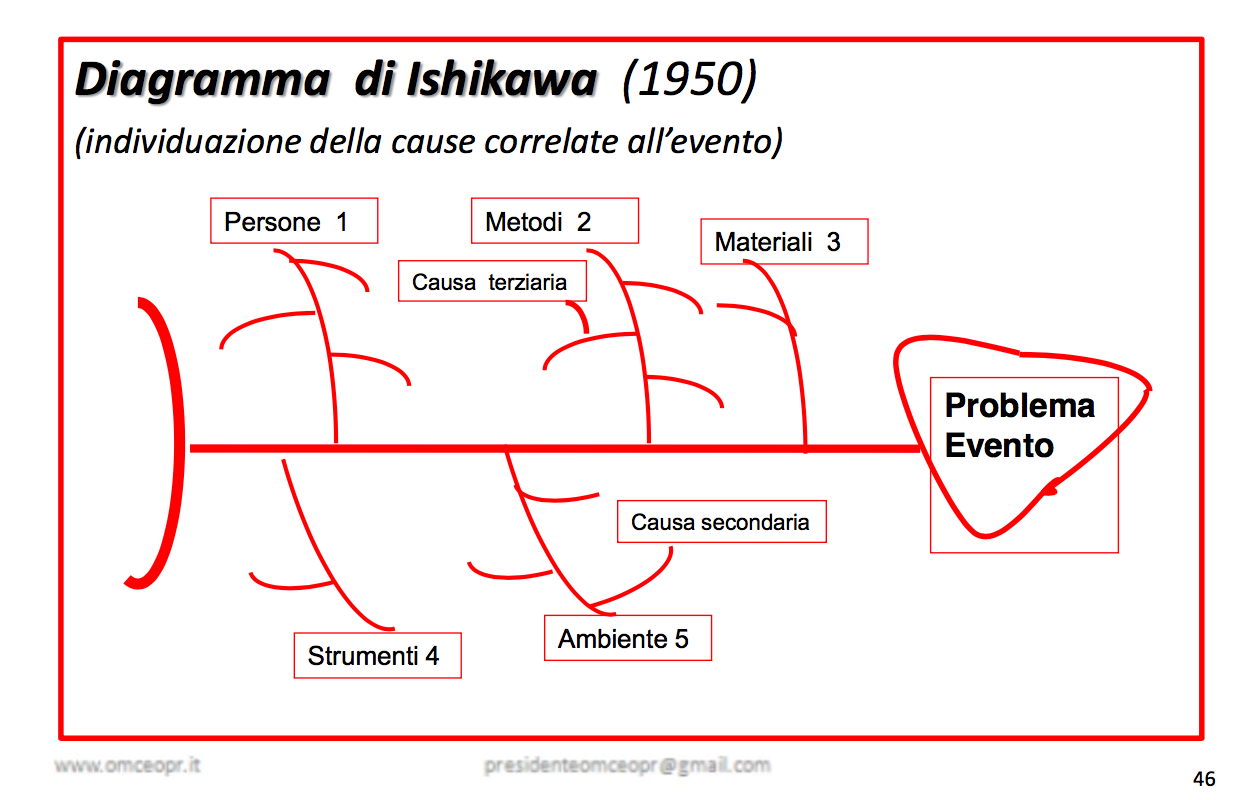
\includegraphics[width=0.8\textwidth]{30/image4.png}
	\end{figure}	
	\emph{Diagramma
  di Ishikawa} permette di scorporare le componenti dell'errore e
  individuare quale sia la possibile causa. Si ricercano le persone
  coinvolte nella procedura incriminata, i metodi usati, i materiali,
  gli strumenti, gli ambienti in cui è avvenuta. L'analisi di tutti
  questi fattori secondo questo diagramma ci porta all'evidenza di dove
  sia stato l'errore che ha prodotto quel problema.
\item
\begin{figure}[!ht]
\centering
	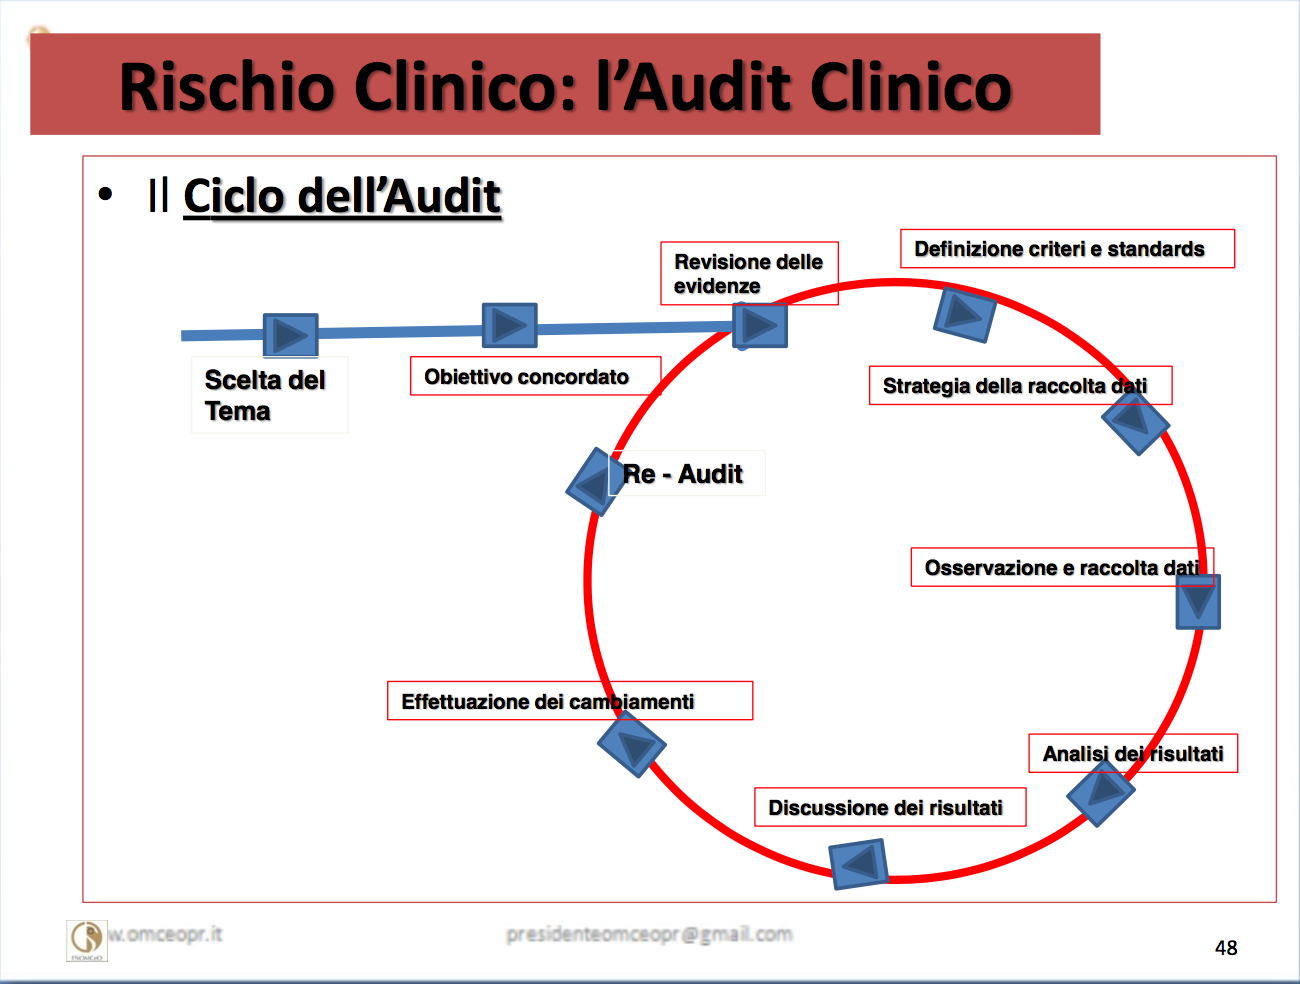
\includegraphics[width=0.8\textwidth]{30/image5.png}
	\end{figure}
  
  \emph{Audit
  clinico}: è una metodologia per andare a rivalutare in modo
  sistematico dove si fanno gli errori.
\end{itemize}

Il \emph{ciclo della qualità} serve per ottenere il massimo della
qualità assistenziale partendo da un tema.\\
Es c'è stato un arresto cardiaco che non abbiamo saputo gestire.
L'obiettivo sarà quello di capire dove si ha sbagliato, per non ripetere
l'errore. Solitamente si vanno consultare le evidenze (linee guida):
``quali sono i percorsi di qualità assistenziale che devono essere messi
in atto?''.\\
Ci dobbiamo dare degli obiettivi, dei criteri, degli standard e dobbiamo
mettere in atto delle strategie. Dobbiamo fare la raccolta dei dati, non
solo quelli di letteratura, ma anche quelli che sono i dati della nostra
attività, per vedere in quali occasioni si sono prodotti i danni.
Infine, dall'analisi dei risultati ridiscutiamo il tema. Ci proponiamo
anche degli obiettivi di cambiamento.

\subsection{Conclusioni}

Il rischio in sanità: rischio ponderabile e rischio imponderabile.

L'errore umano è possibile, se conosciuto può essere evitato e può
servire ad evitare altri errori. L'errore umano deve essere quindi
gestito ed evitato da ciascuno di noi, perché ciò che fa ognuno di noi
può essere un esempio positivo o negativo per la professione.

Non avere paura di segnalare gli eventi avversi, gli errori palesi
commessi in buona fede, i quasi errori commessi o evitati. Cercare di
superare lo stress di aver sbagliato.\\
Vivere la professione non significa vivere in solitudine o
nell'individualità assoluta, bensì mettere in comune il proprio vissuto
personale, ossia le conoscenze e le esperienze personali maturate,
quindi confrontarsi non avendo paura di mettersi in discussione. E
questo è vivere in modo etico la nostra professione.

Qual è il senso di richiamare la deontologia in merito alla gestione
dell'errore? La risposta è in questa frase:

``Ogni atto volto a controllare la salute, che coinvolga i medici con
vantaggio per il paziente, non può che avere un senso etico ed
implicazioni deontologiche. Il controllo del rischio clinico rientra tra
i doveri del medico.''